%!TEX root = thesis.tex
\chapter{Data, Preprocessing and Feature extraction}\label{ch:preprocessing}

\begin{wrapfigure}{r}{7cm}
  \vspace{-35pt}
  \begin{center}
    \newcommand*{\xMin}{0}%
\newcommand*{\xMax}{6}%
\newcommand*{\yMin}{0}%
\newcommand*{\yMax}{6}%
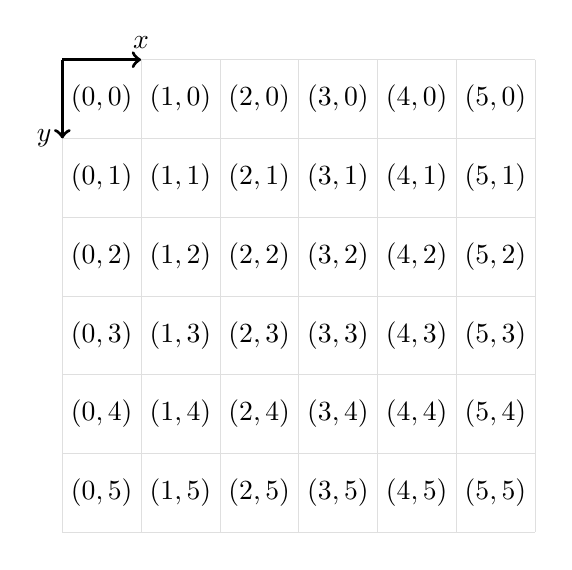
\begin{tikzpicture}[y=-1cm]
    \foreach \i in {\xMin,...,\xMax} {
        \draw [very thin,gray!25] (\i,\yMin) -- (\i,\yMax)  node [below] at (\i,\yMin) {};
    }
    \foreach \i in {\yMin,...,\yMax} {
        \draw [very thin,gray!25] (\xMin,\i) -- (\xMax,\i) node [left] at (\xMin,\i) {};
    }
    \draw[->, very thick] (0,0) -- (1,0) node[above] {$x$};
    \draw[->, very thick] (0,0) -- (0,1) node[left] {$y$};
    \foreach \x in {\xMin,...,5} {
        \foreach \y in {\yMin,...,5} {
            \node at ({\x+0.5},{\y+0.5}) {$(\x, \y)$};
        }
    }
\end{tikzpicture}
  \end{center}
  \vspace{-20pt}
  \caption{HTML5 canvas plane. Each step is one pixel. There cannot be non-integer
           coordinates.}
  \label{fig:canvas-plane}
  \vspace{-10pt}
\end{wrapfigure}

The data that was used for all experiments was collected with
\href{http://write-math.com}{write-math.com}, a website designed solely for
this purpose. This website makes use of HTML5 canvas elements. Those elements
can be used to track fingers or a mouse coursor touching the canvas, moving
and lifting. The origin is at the upper left corner and get bigger to the right
($x$-coordinate) and to the bottom ($y$-coordinate).

The data is stored and shared in JSON format. Each handdrawing is stored as a
list of lines, where each line consists of tuples $(x(t), y(t), t)$, where $x$
and $y$ are canvas coordinates and $t$ is a timestamp in seconds. This timestamp
gives the time in milliseconds from 1970.

The time resolution between points as well as the resolution of the image
depends on the device that was used. However, most symbols have a time
resolution of about $\SI{20}{\milli\second}$ and are within a bounding box of a
$250 \text{px} \times 250 \text{px}$ square.

\section{Preprocessing}\label{sec:preprocessing}
Preprocessing in symbol recognition is done to improve the quality and
expressive power of data. It should make follow-up tasks like segmentation and
feature extraction easier, more effective or faster. It does so by removing
or fixing errors in the input data, reducing duplicate information and
removing irrelevant information.

\subsection{Normalization: Scaling, shifting and resampling}
\textit{Size normalization} is done by many handwriting recognition systems, but
the way in which size normalization is done varies.\\
Single symbol recognizers such as the one presented in \cite{Kirsch} scale the
datapoints to fit into a unit square while
keeping their aspect ratio. Afterwards, the points were shifted to
the $[0, 1] \times [0, 1]$ unit square. The algorithm is given in pseudocode on
\cpageref{alg:scale-and-shift}. It was shown in \cite{Kirsch,Huang09} that
this kind of preprocessing boosts classification accuracy significantly.\\
\cite{Guyon91} shifts the symbol to $[-1, 1] \times [-1, 1]$.

Multiple symbol recognizers such as NPen++ as presented in \cite{Manke01}
scale words in respect to a previously calculated baseline and a corpus line.

Another method to normalize data is \textit{resampling}, sometimes also called
stroke length normalization.
\cite{Guyon91} resampled characters and digits to 81 points each, where different
lines were also connected by \enquote{pen-up} segments. They resampled to get
points regulary spaced in arc length, not in time. \cite{Manke01} also resampled
the points to be equidistant in space, but they used a distance of $\frac{\text{corpus height}}{13}$.
They found an improvement of $5\%$ with this preprocessing step.
\cite{ICASSP-94} also resampled data to get points regulary spaced in arc length, but they encoded
speed as an extra feature.

\subsection{Noise reduction}
The following list of noise reduction techniques was created by \cite{Tappert90}
and is still up-to-date.
\begin{itemize}
    \item \textbf{Dot reduction} reduces dots to single points. Sometimes
          multiple points get recorded although the user wanted to make only
          a single point, e.g. for one of the following symbols:
          $\cdot$, ., $\dots$, $\vdots$, $\ddots$, i, ä, ö, ü.
          This can be detected by calculating
          the maximum distance $d$ two points in a stroke have. If $d$ is
          smaller than a threshold, then it is a single point.
          In that case all points of the line get reduced to a single dot.
          This dot could be the center of mass of all points in the stroke.
    \item \textbf{Dehooking} is the removal of hooks which the author did not
          want to write. Hooks appear sometimes at the end of strokes.
          Examples can be seen in \cref{fig:hooks}. An algorithm in pseudocode
          can be found on \cpageref{alg:dehooking}. A more sophisticated method
          was applied in \cite{Huang09}.
    \item \textbf{Filtering} is the process of removing points by some criteria.
          Those criteria include:
          \begin{itemize}
              \item Duplicate points as applied in \cite{Huang09,Guerfali93},
              \item Enforcing a minimal distance between consecutive 
                    points\cite{Tappert90}.
              \item Maximum velocity / acceleration\cite{Division87}
              \item Enforcing a minimal change in direction\cite{Tappert90}.
          \end{itemize}

          A special reason for the application of filtering methods are occasional spurious points which are also called \textit{wild points}.
    \item \textbf{Smoothing} can be done in multiple ways. An approach that was
          used quite often is applying a weighted average
          \cite{Groner66,Division87,Arakaw83}. \Cref{alg:weighted-average-smoothing}
          describes in pseudocode how weighted average smoothing can be implemented.
    \item \textbf{Stroke connection} might be used if the distance between
          pen-up and pen-down is below a threshold. \cite{Guerfali93} describes
          that such maliciously disconnected components can get detected by
          observing angular continuity and the shortness of distance between
          two strokes.
    \item \textbf{Deskewing} corrects character slant. Although this technique
          was applied by some authors \cite{Bozinovic1989,Guerfali93,IWFHR94},
          it seems not ot be
          applicable to the domain of mathematical handwriting, because on the
          one hand symbols might occur in variations with slant, like
          $\rightarrow$ and $\nearrow$. On the other hand it is questionable
          if slant is as consistent with symbols as it is with cursive
          handwriting.
    \item \textbf{Baseline drift correction} moves words to be on a baseline.
\end{itemize}

An idea for filtering that seemingly nobody has tried before is applying the
Douglas-Peucker algorithm.

\begin{figure}[ht]
    \centering
    \subfloat[Hook at the end of $\hbar$]{
        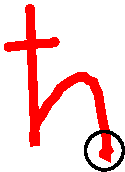
\includegraphics[height=0.3\linewidth, keepaspectratio]{figures/8350.pdf}
        \label{fig:hook-hbar}
    }%
    \subfloat[Hook in the letter R]{
        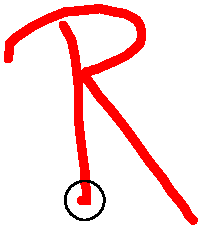
\includegraphics[height=0.3\linewidth, keepaspectratio]{figures/11387.pdf}
        \label{fig:hook-R}
    }%
    \caption{Examples for hooks}
    \label{fig:hooks}
\end{figure}

\section{Features}\label{sec:features}
A number of different features have been suggested so far for on-line handwriting
recognition. They can be grouped into local features and global features.
Local features apply to a given point on the drawing plane and sometimes even
only to point on the drawn curve whereas global features apply to a complete
line or even the complete image.

\subsection{Local features}
\begin{itemize}
    \item \textbf{Coordinates} of the current point are used by \cite{Guyon91}.
    \item \textbf{Speed} has been used by \cite{ICASSP-94}, but
          \cite{Kosmala98,Kosmala11} suggest that speed is a bad feature,
          because they think that speed is \enquote{highly inconsistent}.
    \item \textbf{Binary pen pressure} has been used by \cite{Kosmala98,Kosmala11,ICASSP-94,Manke94,Guyon91}.
    \item \textbf{Direction} has been used by \cite{Manke95,Huang06}.
The \textbf{direction} at the point $i$ can be described by the vector 
$(\cos \theta(i), \sin \theta(i))$ as described in \cite{Guyon91}:
\begin{align}
    \cos \theta(i) &= \frac{\Delta x^{(i)}}{\Delta s^{(i)}}\\
    \sin \theta(i) &= \frac{\Delta y^{(i)}}{\Delta s^{(i)}}
\end{align}
where
\begin{align}
    \Delta x (i) &= x^{(i+1)} - x^{(i-1)}\\
    \Delta y (i) &= y^{(i+1)} - x^{(i-1)}\\
    \Delta s (i) &= \sqrt{(\Delta x(i))^2 + (\Delta y (i))^2}
\end{align}
    \item \textbf{Curvature} has been used by \cite{Groner66,Manke95,ICASSP-94,Guyon91}.
          It is calculated in \cite{Guyon91} by the angle of two neighboring
          lines like this:
          \begin{align}
              \varphi(i)      &= \theta(i+1) - \theta(i-1)\\
              \cos \varphi(i) &=\cos \theta (i-1) \cdot \cos \theta (i+1)\\
                              &+\sin \theta (i-1) \cdot \sin \theta (i+1)\\
              \cos \varphi(i) &=\cos \theta (i-1) \cdot \cos \theta (i+1)\\
                              &-\sin \theta (i-1) \cdot \sin \theta (i+1)
          \end{align}
    \item \textbf{Bitmap-environment} has been used by \cite{Manke94}make. This
          feature is a $3 \times 3$ pixel environment around the current point.
          It allows the recognizer to determine points that cross or touch
          strokes. 
    \item \textbf{Hat-Feature} has been used by \cite{ICASSP-94,Manke00}.
\end{itemize}


\subsection{Global features}
\begin{itemize}
    \item \textbf{Re-curvature} is defined in \cite{Huang06,Huang09} as the
          ratio between the height of a stroke and the distance between its
          start and end points.
    \item \textbf{Center point} was used in \cite{Huang06}.
    \item \textbf{Stroke length} was used in \cite{Huang06}. It can be
          calculated by using a linear interpolation.
    \item \textbf{Number of strokes} was used in \cite{Huang09}.
    \item \textbf{Sequence features}
    \begin{itemize}
        \item \textit{Pentip sequence}: \cite{Kirsch} used the raw pentip
              sequence combined with \gls{DTW} to recognize mathematical symbols.
              Other authors like \cite{Koschinski95} used pentip sequences, too,
              but made use of \glspl{HMM} or \glspl{ANN} to recognize symbols
        \item \textit{Zone sequences} are used by \cite{Brown1964,Hanaki80}. The
          idea is to recognize symbols by dividing the box in which the
          character is written into zones. By examining the position of the
          pen-tip a sequence of zones can be generated for a written symbol.
        \item \textit{Direction sequences} were used in \cite{Impedovo1976,Powers1973}.
    \end{itemize}
\end{itemize}

There are other global features used for off-line handwriting recognition which
I will not examine. Examples are Pseudo-Zernike moments and Shadow Code features
which were used in \cite{Khotanzad}.